\documentclass[12pt]{ctexart}
\makeatletter
\usepackage{amsmath}
\usepackage{amsfonts}
\usepackage{ctex}
\usepackage{bm}
\usepackage{graphicx}
\usepackage{diagbox}
\usepackage{subfigure}
\usepackage{multirow}
\usepackage{geometry}
\usepackage{caption} 
\usepackage{fancyhdr}
\usepackage{minted}
\usepackage{cite}
\usepackage{hyperref}
\hypersetup{hidelinks} 
\geometry{a4paper,left=3cm,right=3cm,top=3cm,bottom=3cm}
\pagestyle{fancy}
\lhead{{\songti 吉林大学学士学位论文}}
\chead{}
\rhead{\leftmark}

\begin{document}
\bibliographystyle{unsrt}
\thispagestyle{plain}
\pagenumbering{Roman}
\section*{摘要}
随着传感器技术的发展, 多元时间序列数据已经可以广泛地获取. 所以怎样提取多元时间序列中的信息是近几年机器学习领域中的重点问题和高价值问题. 传统的方法需要手动选择特征, 而更为先进的方法可以自动学习和提取特征. 本文采用了拓扑数据分析(TDA), 卷积神经网络(CNN), 和长短期记忆网络(RNN with LSTM)模型. 并通过14个传感器记录的脑电图时间序列数据比较了3种模型的优劣. 结果表明, 长短期记忆网络在处理多元时间序列数据时表现得较好.所有的数据和源代码均于\url{https://github.com/HaiyangYu1999/CodeBackup/tree/master/python/MTSC}可见.
\newline
\newline
\textbf{关键词:}\ 多元时间序列,\ 拓扑数据分析,\ 卷积神经网络,\ 长短期记忆网络
\section*{Abstract}
\noindent With the advance of sensor technology, multivariate time series data can be approached widely. Thus, extraction information from Multivariate Time Series has been one of the most essential problems in machine learning community in the recent decades. Traditional methods employ hand-crafted features for classification while the cutting edge technologies we use could auto-recognize and auto-extract these features. In this paper, we implement Topological Data Analysis (TDA), Convolution Neural Network (CNN) and Recurrent Neural Network with Long Short Term Memory (RNN with LSTM) model. Then evaluate the three models based on a dataset about electroencephalogram (EEG) recorded by 14 sensors. The result shows that RNN with LSTM prevails in the dataset. All the data and codes are available at \url{https://github.com/HaiyangYu1999/CodeBackup/tree/master/python/MTSC}.
\newline
\newline
\textbf{Keywords:}\ Multivariate Time Series Classification,\ Topological Data Analysis,\ Convolution Neural Network,\ Long Short Term Memory

\newpage
\thispagestyle{plain}
\setcounter{page}{1}
\tableofcontents
\newpage
\pagenumbering{arabic}
\setcounter{page}{1}
\section{绪论}
\subsection{研究背景和意义}
时间序列是一组按时间排序的实际观察值. 而多元时间序列是一组由多个传感器在相同的时间戳下同时记录的多组数据序列. 随着传感器技术的发展, 时间序列的分类问题, 即从时间序列中鉴别所属类别的问题, 在近十几年受到了广泛的关注. 因为时间序列数据广泛地存在于研究领域和应用领域, 所以时间序列模型被应用于多种多样的实际问题中, 例如, 人体行为识别\cite{ref1}, 脑电图数据分析\cite{ref2}, 声音识别\cite{ref3}. 

早期对于时间序列的研究方法主要集中在数学方法和统计方法上. Kleinbaum等和Kurth等讨论了logistic回归和其他广义线性模型(GLM)在处理多元时间序列数据中的应用\cite{ref4,ref5}. Tiwari等利用傅立叶分析预测了DNA序列中可能出现的基因\cite{ref6}. Mabrouk等使用小波分解和ARMA模型讨论了时间序列的预测问题\cite{ref7}. 在经济学和社会学时间序列的研究中, VAR模型和SVAR模型仍然占据优势\cite{ref8,ref9,ref10}. Rabiner使用隐式Markov模型来识别语音信息\cite{ref11}. 

传统的数学和统计方法注重变量之间的关系, 有着十分严谨的理论基础, 即使是最坏条件下性能和误差也可得到保障. 但是处理非线性数据能力较差或需要手动选择特征, 要求使用者有较多的先验知识. 而最近兴起的机器学习方法更偏向于启发性算法, 强调从数据中学习某种特征, 有着较强的处理复杂非线性数据的能力, 可以通过大量的数据自动学习并提取特征, 但是全局最优性无法保证. 随着计算能力的提高, 越来越多的机器学习方法被提出用来预测时间序列, 例如人工神经网络\cite{ref12}和支持向量机\cite{ref13}.

\subsection{研究现状}
如上所诉, 对于时间序列的研究, 机器学习方法占据主流, 也有许多机器学习方法与传统统计方法结合的模型, 并且都取得了不错的结果. Zhang, G. P.提出了将ARIMA模型与神经网络结合的方法\cite{ref14}. Hassan Ismail Fawaz等总结了神经网络预测时间序列的一般方法\cite{ref28}. Yazdanbakhsh等使用了复杂模糊神经网络预测多元时间序列\cite{ref16}. Orozco采用了长短期记忆的循环神经网络预测时间序列\cite{ref17}. Ignatov使用卷积神经网络来识别人类的运动行为\cite{ref18}. L.-J. Cao等使用了含自适应参数的支持向量机预测金融时间序列\cite{ref19}. Z. Che等讨论了含有缺失数据下的时间序列问题\cite{ref20}. 

此外, 从其他领域借鉴的其他方法在时间序列的预测中也取得了出色的结果. Farmer等利用微分方程理论来预测混沌时间序列\cite{ref21}, Wu等依据持续同调理论, 利用房间传感器的时间序列信息预测房间中是否有人活动\cite{ref22}. Koop等运用贝叶斯理论预测宏观经济学中的多元时间序列\cite{ref23}. Wu等将基于遗传算法优化的残差神经网络用于时间序列的分类问题\cite{ref24}.
\subsection{研究内容}
本文讨论并实现了从多元时间序列中提取特征的3种方法, 分别是拓扑数据分析(TDA), 卷积神经网络(CNN)和长短期记忆网络(RNN with LSTM). 采用脑电图(EEG)时间序列数据作为本文的数据集. 将80\%的数据作为训练集, 20\%的数据作为测试集. 经过归一化(Standardization)后的数据会被用于训练和评价各个模型. 本文使用二分类问题中的准确率(accuracy), 敏感性(sensitivity), 特异性(specificity)作为评价各个模型的指标. 结果表明, 长短期记忆网络在处理多元时间序列数据时表现得较好.

\subsection{论文结构}

本文在分析目前常用的时间序列数据的分类和预测方法的基础上, 选用较为常用的3个模型(拓扑数据分析, 卷积神经网络和长短期记忆网络)和相同的数据集进行实验. 本文的主要结构如下:

第一章主要介绍了研究时间序列问题的背景和意义, 研究现状, 本文主要的研究内容, 和本文的结构.

第二章主要介绍了多元时间序列分类方法的定义, 数据预处理, 本文用到的模型及其相关的理论知识.

第三章介绍了所选用的数据集, 然后使用相同的训练集训练选用的3个模型, 用相同的测试集的预测结果作为模型的评价结果.

第四章根据评价的3个指标(准确性, 灵敏性, 特异性)评价所选用模型的优劣, 并分析准确性差异的原因.


\newpage
\section{预测模型相关理论}
\subsection{多元时间序列分类问题} \label{lb1}
一个多元时间序列(MTS) $X=\{\bm{x}_{1},\cdots,\bm{x}_{m}\}\in \mathbb{R}^{l × m}$是一列关于向量$\bm{x}_{i}=(x_{1,i},\cdots,x_{l,i})^{\mathrm{T}}$的向量序列. 其中, $l\in \mathbb{N}$ 是时间序列$X$的长度, $m\in \mathbb{N}$是多元时间序列$X$的维度. 例如, 当一个灰尘传感器收集了100条按照时间顺序的三维(PM1, PM2.5和PM10)记录, 这个多元时间序列就可以用一个维数为3, 长度为100的矩阵代替. 

每个多元时间序列都与一个类别标签$y\in \Omega$相关联. 其中, $\Omega$为事先定义好的类别集合. 给定一组多元时间序列
$\mathcal{X}=\{X_{1},\cdots,X_{n}\}\in \mathbb{R}^{n × l × m}$
($n$为多元时间的数量), 和对应的类别标签$\bm{y}=\{y_{1},\cdots,y_{n}\}\in \Omega^{n}$. 多元时间序列分类的任务就是训练一个分类器$f_{\mathcal{X}}\mapsto \bm{y}$来预测一个未知标签的多元时间序列的类别\cite{ref12}.
\subsection{数据归一化}\label{lb2}
在分割数据为训练集和测试集后, 按照机器学习领域中的一般方法,我们首先进行数据归一化使得多元时间序列中的每一个特征拥有0均值和单位方差. 这样做的好处是避免因为一个特征因数值太大而相对其他特征占据支配地位. 为了避免训练集和测试集相关, 保证客观性, 使用训练集的均值和方差归一化全部的数据集. 算法如下:
$$x_{ij}^{'}=\frac{x_{ij}-\mathrm{E}(x_{j}^{\mathrm{train}})}{\sqrt{\mathrm{Var}(x_{j}^{\mathrm{train}})}}$$
\subsection{拓扑数据分析}\label{lb3}
拓扑数据分析(TDA)是一种使用拓扑技术对数据集进行分析的方法, 从高维, 不完整和嘈杂的数据集中提取信息. 其最初的动机是研究数据的形状. TDA已将代数拓扑与纯数学中的其他工具结合在一起, 可以对``形状"进行严格的数学研究. 主要工具是持续同调, 即对点云数据的同调转换.

\subsubsection{点云}

我们将采用Gidea\cite{ref25}的方法将多元时间序列转化为点云. 同时, 引入一个新的变量$s$, 代表步长. 考虑一个$d$维的多元时间序列$\{x_{n}^{k}\}_{n}, k=1,\cdots, d$. 固定一个滑动窗口大小$w$.对于每个时刻$t_{n}$, 我们定义$\mathbb{R}^{d}$中的点$x(t_{n})=(x_{n,1},\cdots,x_{n,d})$.因此, 对于每个窗口大小$w$, 我们得到包含$w$个点的点云
$$X_{n}=(x(t_{1+s(n-1)}),x(t_{2+s(n-1)}),\cdots,x(t_{w+s(n-1)}))$$
简要来说, 滑动窗口大小$w$决定了点云中有多少点, 步长$s$决定了隔多少步选取一次点云. 在本文中, 我们取$w=s=10$.
\subsubsection{消除对称性和锚点}
在传统的拓扑数据分析中, 每个坐标轴扮演相同的角色并且有同样的重要性. 比如, 在$\mathbb{R}^{3}$中, $x, y, z$坐标轴被同等的对待. 这种特性使得拓扑数据分析方法在处理3D图像的时候表现更加出色. 但是, 对于处理多元时间序列问题, 这种特性变成了阻碍. 例如, 拓扑方法不能分辨出以下两个点云
$$X_{1}=\{(0,0,0),(0,0,1)\},$$
$$X_{2}=\{(0,0,0),(0,1,0)\},$$
因为每个点云之间的点的距离是一样的(都为1). 对于多元时间序列来说这可能是一个关键性的问题, 因为不同的坐标轴或许代表不同的特征. 

在这里, 本文引入两个基本的技术. 消除对称性和锚点. 消除对称性是指对每个$\mathbb{R}^{d}$中的点添加一个固定的常数向量. 而锚点是指在点云这个集合中加入一个固定的点. 我们定义如下,

\textbf{对称性消除}: 设$X$是含有$\mathbb{R}^{d}$中的点的点云, 令$\bm{v}=(c_{1},c_{2},\cdots,c_{n})\in \mathbb{R}^{d}$为一个固定的向量, 定义消除对称性后的点云
$$X'=\{\bm{x}+\bm{v}|\bm{x}\in X \}.$$

\textbf{锚点}: 设$X$是含有$\mathbb{R}^{d}$中的点的点云, 定义锚点$A$为一组在$\mathbb{R}^{d}$中的点的集合
$$A=\{\bm{a_{1}},\bm{a_{2}},\cdots,\bm{a_{n}}\},\ \bm{a_{i}}\in \mathbb{R}^{d}$$
定义新的点云$Y=X'\cup A$. 在上面的例子中, 我们选取
$\bm{v}=(0,1,2), A=\{(0,0,0)\}$. 因此新的点云
$$Y_{1}=X_{1}'\cup A=\{(0,1,2),(0,1,3),(0,0,0)\}$$
$$Y_{2}=X_{2}'\cup A=\{(0,1,2),(0,2,2),(0,0,0)\}$$
我们注意到, 在新的点云中, $(0,1,3)$到$(0,0,0)$的距离为$\sqrt{10}$,而$(0,2,2)$到$(0,0,0)$的距离为$2\sqrt{2}$. 因此, TDA算法现在可以正确识别点云$Y_{1}$和$Y_{2}$之间的差异了.
\subsubsection{持续图}


持续图是$\mathbb{R}^{2}$中一列点的集合$\{(b,d)|(b,d)\in \mathbb{R}^{2}\ \mathrm{and}\  d>b\}$, 对应着相应的单纯复形的拓扑特性\cite{ref22,ref26}. 特别的是, 每一个点$(b,d)$表示着以半径$b$出生, 以半径$d$``死亡"的拓扑特征. 这里, ``死亡"可以看作一个同调特征被更低维度的单纯形填充满. 一个特征的持续性被定义为$d-b$, 被解释为一个拓扑特征在它被填充满之前的持续时间. 例如, 在图 \ref{fig1} 左图中, 我们期望在相对较小的半径形成一个洞, 并且这个孔会持续很长时间. 这对应了持续图(图 \ref{fig1} 右图)中的点(0.65,7.9). 

\begin{figure}[H]
  \centering
  \subfigure[point cloud]{
    \label{fig:subfig:onefunction} 
    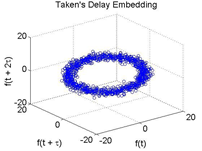
\includegraphics[scale=.8]{1.png}}
  \hspace{0.5in} 
  \subfigure[persistence diagram]{
    \label{fig:subfig:twofunction} 
    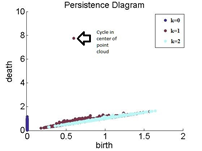
\includegraphics[scale=.8]{2.png}}
  \caption{左图是在$\mathbb{R}^{d}$中的点云. 右图是对应的持续图. 图片来自\emph{Data Analysis Methods using Persistence Diagrams}\cite{ref26}.}
  \label{fig1}
  \label{fig:twopicture} 
\end{figure}
\subsubsection{Wasserstein距离}
简要来说, 持续图可以被看作点云的持续同调的可视化表示\cite{ref22}. 为了衡量各个点云对应的持续图的差异,  我们引入Wasserstein 距离. 两个持续图$D_{1},\ D_{2}$的$p$-Wasserstein距离定义为
$$W_{p}(D_{1},D_{2})=\left(\inf_{\varphi:D_{1}\rightarrow D_{2}}\sum_{x\in D_{1}}||x-\varphi(x)||^{p}_{\infty}\right)^{\frac{1}{p}},$$
其中, $\varphi$是所有从$D_{1}$到$D_{2}$之间的双射. 在本文中, 我们取$p=1$, 即搬土距离(earth mover's distance). 此距离在计算机科学领域中被广泛的应用于比较两个离散分布的差异.

\subsubsection{$k$邻近算法}
为了得到测试集中时间序列对应的分类标签, 运用基于Wasserstein距离的$k$邻近算法($k$-NN). 对于测试集中的任一一个点云$X$, 我们通过$k$-NN算法确定距离$X$最近的$k$个训练集中的点云$\mathcal{Y}=\{Y_{1},Y_{2},\cdots,Y_{k}\}$, 将$\mathcal{Y}$中点云的多数类别标签作为点云$X$的类别标签.


\subsection{卷积神经网络}
\label{lb4}
卷积神经网络(CNN)是一类深度神经网络, 最常用于分析视觉图像. 同时在图像和视频识别, 推荐系统, 图像分类, 医学图像分析, 自然语言处理, 和财务时间序列中也都有应用.
卷积神经网络由输入层, 输出层和多个隐层组成. 隐层通常由一系列激活函数为ReLu的卷积层组成, 随后是池化层, 完全连接层和归一化层.

\subsubsection{序列预处理}

卷积神经网络的输入是用一个四维元组 \mintinline{c}|(batch,length,width,channel)| 描述的图片集合. 其中, \mintinline{c}|batch| 为每批处理的图片数量, \mintinline{c}|length| 和 \mintinline{c}|width| 为每张图片的像素长度和像素宽度, \mintinline{c}|channel| 为通道数. (例如, 普通的彩色图片是由RGB 3种颜色的像素矩阵组成的, 此时通道数就为3.)

 对于一组多元时间序列$\mathcal{X}=\{X_{1},\cdots,X_{n}\}\in \mathbb{R}^{n × l × m}$ (定义见\ref{lb1}), 将多元时间序列的数量$n$看作批处理数量, 长度$l$和维数$m$代替图片中的像素长度和像素宽度. 通道数设为1. 简要来说, 就是将代表多元时间序列的矩阵看作代表图片的矩阵来处理\cite{ref29}, 后续步骤与处理图片的过程完全一致.

\subsubsection{卷积层}
卷积层是CNN最重要的核心组成部分. 其参数由一组可学习的卷积核组成, 这些卷积核的视野较小, 但会扩展到输入体积的整个深度. 在前向传播期间, 每个卷积核会在输入体积的宽度和高度上卷积, 并生成该过滤器的二维激活图. 

\begin{figure}[H]
  \centering
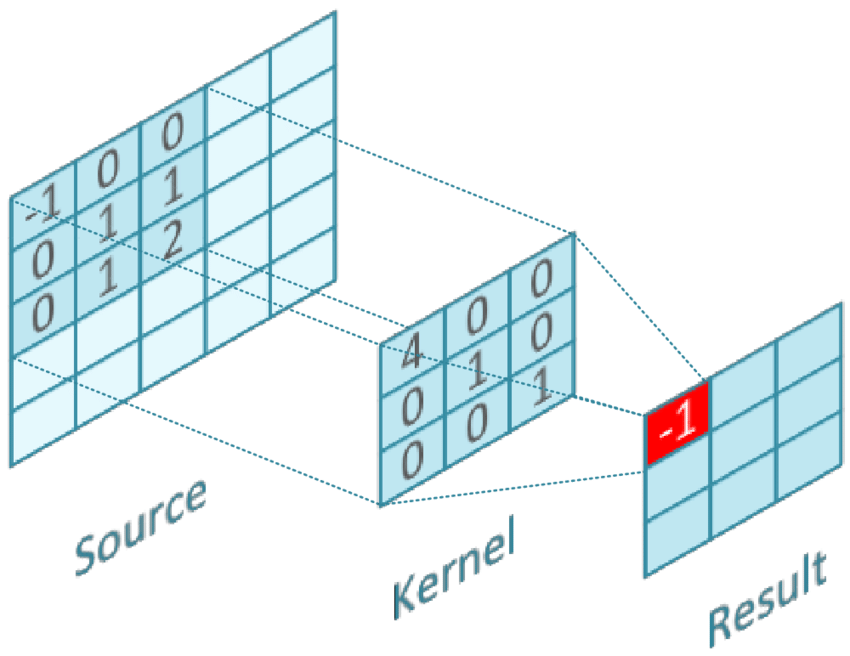
\includegraphics[scale=.15]{7.png} 
\caption{Convolution with a $3\times3$ kernel. Figure is from \url{https://www.researchgate.net/}.}
\label{fig4}
\end{figure}
需要注意的是, 这里的卷积并不是指数学意义上的卷积, 而是和矩阵内积相似的运算(如图 \ref{fig4} 所示). 设卷积核$K=(k_{ij})_{F \times F}$(这里的$F$通常被称为感受野, 通常选取$F=3$或$F=5$), 与卷积核对应相同位置的像素矩阵$A=(a_{ij})_{F\times F}$. 两者卷积的定义为
$$\mathrm{Convolution}(A,K)=\sum_{i=1}^{F}\sum_{j=1}^{F}a_{ij}k_{ij}.$$

当大小为$F\times F$的卷积核$K$以步长$S$遍历大小为$W_{1}\times W_{2}$的输入图片后, 便得到了一个大小为$P_{1}\times P_{2}$的输出矩阵$O$. 其中, 输出矩阵的大小由图片大小, 卷积核感受野和步长共同决定(暂不考虑边缘填充). 
$$P_{i}=\frac{W_{i}-F}{S}, \ i=1,2.$$

对于多通道图片(设通道数 \mintinline{c}|channel| 为$c$), 各个特征通常是存在于不同的通道中,(例如, 对于手写数字的RGB 3通道图像, 数字``8"的上半部分为红色而下半部分为蓝色, 此时单一的卷积核就不能正确识别) 为了将多个通道中提取的特征碎片合并, 则需要设置$c$个卷积核. 这些卷积核的集合定义为过滤器$\mathcal{K}=\{K_{1},\cdots,K_{c}\}$.
将过滤器中的每个卷积核与其对应的通道分别做卷积, 得到$c$个输出矩阵$O_{i}\in \mathbb{R}^{P_{1}\times P_{2}},\ i\in \mathbb{Z}_{c}$.将这些输出矩阵相加并加上一个偏置系数$b\in \mathbb{R}$, 得到这个过滤器$\mathcal{K}$的过滤结果
$$V=\sum_{i=0}^{c-1}O_{i}+b,\ V\in \mathbb{R}^{P_{1}\times P_{2}}.$$
其中, 矩阵与标量的加法被定义为矩阵的每一个元素与标量相加.

一般来说, 我们期望在一张图片中提取多个特征, 这时就需要多个过滤器. 假设在一层卷积层中有$n$个过滤器, 则每一个过滤器$\mathcal{K}_{i},\ i\in \mathbb{Z}_{n}$和它对应的偏置系数$b_{i},\ i\in \mathbb{Z}_{n}$作用于输入图片得到卷积的输出$V_{i},\ i\in \mathbb{Z}_{n}$, 经过激活函数激活后得到神经元的输出$\mathrm{relu}(V_{i}),\ i\in \mathbb{Z}_{n}$. 其中, $\mathrm{relu}(x)=\max(0,x)$, $\mathrm{relu}(V)=(\mathrm{relu}(v_{ij}))_{P_{1}\times P_{2}}$.

 至此, 我们已经得到卷积层的所有输出$\mathcal{V}=\{\mathrm{relu}(V_{0}), \cdots, \mathrm{relu}(V_{n-1})\}$和卷积层的所有参数$\mathfrak{K}=\{(\mathcal{K}_{0},b_{0}), \cdots, (\mathcal{K}_{n-1},b_{n-1})\}$.
输出$\mathcal{V}$将作为下一个神经元的输入, 而参数$\mathfrak{K}$将会在迭代的过程中不断被训练.

\subsubsection{池化层}
CNN的另一个重要层是池化层, 其中最大值池化是最常见的. 它将输入图像划分为一组不重叠的矩形(正方形), 并为每个此类子区域输出最大值. 池化层的作用是逐渐减小表示的空间大小, 减少参数的数量, 减少内存占用以及网络中的计算量, 并因此也控制过拟合. 
设池化层的大小为$n\times n$(以$2\times 2$最为常见), 输入为矩阵$S$, 则池化池的输出可以表示为(如图 \ref{fig2} 所示):
$$f_{x,y}(S)=\max_{a,b\in \mathbb{Z}_{n}} S_{nx+a,ny+b}.$$ 
\begin{figure}[H]
  \centering
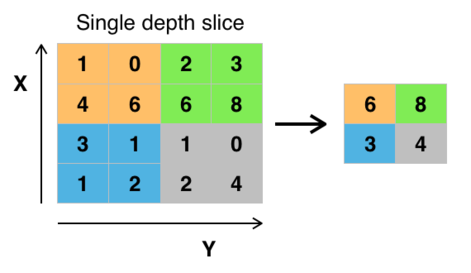
\includegraphics[scale=.5]{5.png} 
\caption{Max pooling with a $2\times 2$ filter. Figure is from Wikipedia.}
\label{fig2}
\end{figure}

\subsubsection{全连接层}
经过几个卷积层和最大池化层之后, 卷积神经网络是通过完全连接的层结束的. 和常规人工神经网络一样, 全连接层中的神经元与上一层中的所有神经元都有连接. 全连接层的作用是计算并输出一个分类标签的概率向量, 并由此预测最终的分类结果. CNN的结构如图 \ref{fig3} 所示.
\begin{figure}[H]
  \centering
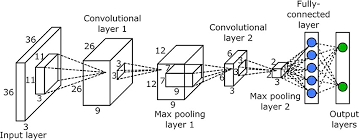
\includegraphics[scale=.8]{6.png} 
\caption{CNN Architecture. Figure is from \url{https://mc.ai/}.}
\label{fig3}
\end{figure}


\subsection{长短期记忆网络}
\label{lb5}
递归神经网络(RNN)是一类人工神经网络, 其中节点之间的连接沿时间序列形成有向图. 这使其表现出时间动态行为. RNN源自前馈神经网络, 可以使用其内部状态(内存)来处理可变长度的输入序列\cite{ref30}. 这使得它们适用于诸如连续的手写识别\cite{ref31}或语音识别之类的任务\cite{ref32}.

长短期记忆(LSTM)是一种递归神经网络(RNN)扩展, 是为了解决训练传统RNN时可能遇到的梯度消失问题. 
常见的LSTM神经元含有输入门, 输出门和忘记门. 并且三个门控制着进出单元的信息流. LSTM网络非常适合时间序列数据的分类, 处理和预测. 因为时间序列中重要事件之间可能存在未知持续时间的滞后, 而LSTM的结构使得它可以记住任意时间间隔内的值.

长短期记忆网络中每一个神经元的结构如图 \ref{fig5} 所示.
\begin{figure}[H]
  \centering
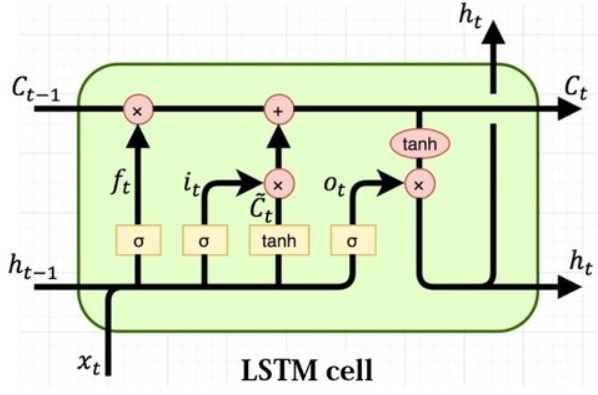
\includegraphics[scale=.4]{8.png} 
\caption{Structure of the LSTM cell. Figure is from \url{https://www.researchgate.net/}.}
\label{fig5}
\end{figure}
\subsubsection{输入门}
可以看出, LSTM较普通的RNN增添了一个单元状态$C_{t}$的变量. 该变量的记录了前$t$个神经元的状态. $\bm{h}_{t-1}$为上一个LSTM神经元的输出, $\bm{x}_{t}$为神经元的输入(上一层神经元的输出), $\bm{h}_{t}$为这个神经元的输出(作为下一个神经元的输入和下一层神经元的输入). 以下假定输入$\bm{h}_{t-1}$和$\bm{x}_{t}$均为同维数的列向量, 其他变量均为维数与之匹配的向量或矩阵.
\subsubsection{忘记门}
在前向传递的过程中, 第$t$个神经元接受上一个神经元的输出$\bm{h}_{t-1}$, 前$t-1$个神经元的单元状态$C_{t-1}$, 和来自上一层的输入$\bm{x}_{t}$. 首先, 对于来自前$t-1$个神经元的单元状态, 第$t$个神经元根据输入$\bm{h}_{t-1}$和$\bm{x}_{t}$决定应当``记住"或``忘记"前$t-1$个神经元的单元状态$C_{t-1}$中的哪些内容$f_{t}$.
$$f_{t}=\sigma (W_{f}\cdot (\bm{h}_{t-1},\bm{x}_{t})+\bm{b}_{f})$$ 
$$B_{t-1}=f_{t}\odot C_{t-1}$$
其中, $B_{t-1}$表示忘记了某些内容后的前$t-1$个神经元的单元状态, $\sigma$为Sigmoid激活函数(下同), $W$和$\bm{b}$为相应的权重矩阵和偏置系数(下同), $\odot$表示矩阵的Hadamard积(下同).

接下来, 要确定这一个神经元的神经元状态. 这分为两步, 首先, 要根据输入$\bm{h}_{t-1}$和$\bm{x}_{t}$计算神经元状态$\tilde{C}_{t}$, 其次, 要计算$i_{t}$决定哪些信息需要``忘记", 哪些信息需要``记住"并传给后面的神经元.
$$\tilde{C}_{t}=\mathrm{tanh}(W_{C}\cdot (\bm{h}_{t-1},\bm{x}_{t})+\bm{b}_{C})$$
$$i_{t}=\sigma(W_{i}\cdot (\bm{h}_{t-1},\bm{x}_{t})+\bm{b}_{i})$$

然后, 将忘记了某些信息后的前$t-1$个神经元的状态$B_{t-1}$和记录了某些需要传递的信息的当前神经元状态$i_{t}\odot \tilde{C}_{t}$作为前$t$个神经元的状态$C_{t}$传递给后面的神经元.
$$C_{t}=B_{t-1}+i_{t}\odot \tilde{C}_{t}$$
\subsubsection{输出门}
最后, 根据$C_{t}$, $\bm{x}_{t}$和$\bm{h}_{t-1}$确定这个神经元的输出$\bm{h}_{t}$.
$$o_{t}=\sigma(W_{o}\cdot (\bm{h}_{t-1},\bm{x}_{t})+\bm{b}_{o})$$
$$\bm{h}_{t}=\mathrm{tanh}(C_{t}).$$
至此, 完成了数据前向传递的过程.


\section{实验}
\subsection{数据介绍}
本文研究了关于脑电图(EEG)的多元时间序列数据. 数据来源为加州大学尔湾分校机器学习仓库(UCI Machine Learning Repository) \url{http://archive.ics.uci.edu/ml/datasets/EEG+Eye+State}. 所有数据均来自使用 Emotiv EEG 的神经耳机的连续 EEG 测量. 测量持续时间为 117 秒. 在 EEG 测量期间, 通过摄像机检测眼睛状态, 并在分析视频帧后手动添加到文件中. ``1"表示闭眼状态, ``0"表示睁眼状态, 所有值按时间顺序排列, 并且第一个测量值在数据顶部. 

在数据集中, 前14列均为神经耳机传感器(AF3, F7, FC5等14个)在同一时刻记录的不同位置的脑电图状态, 最后1列为摄像机在相同时刻记录的眼睛状态. 而每一行代表某一时刻的一条记录, 共有14980条. 所以, 在此数据集中$d=14, l=14980$(符号说明见 \ref{lb1}). 对于所有的模型, 均将前80\%的数据(11980行)作为训练集, 后20\%的数据(3000行)作为测试集. 并采用相同的方法归一化(\ref{lb2}节). 

\subsection{拓扑数据分析}
\subsubsection{实验步骤}
我们完全按照 \ref{lb3} 中讨论的步骤进行. 

选取$w=s=10$, 因此, 每个点云中的时间窗口不重叠. 每个点云中(不包含锚点)含有10个在$\mathbb{R}^{14}$中的点. 使用固定的向量$\bm{v}=(0,1,2,\cdots,13)$破坏对称性, 使用锚点$A=\{(0,0,\cdots,0)\}$. 

对于每个点云对应的持续图, 我们通过R语言 \mintinline{c}|TDA| 包中的 \mintinline{c}|ripsDiag| 函数来计算. 为了计算两个持续图的1-Wasserstein距离, 使用R语言 \mintinline{c}|TDA| 包中的 \mintinline{c}|wasserstein| 函数来计算. 最后, 选取$k=10$, 使用$k$-NN算法来预测测试集点云的类别标签. 
\subsubsection{缩短计算时间}
为了缩短计算时间, Wu Chengyuan等没有选择计算任意两个持续图的距离, 而是计算测试集任一持续图到训练集任一持续图的距离, 这大概减少了68\%的计算量\cite{ref22}. 

在Wu Chengyuan等的基础上, 可进一步缩短计算时间. 观察到在迭代过程中发生了大量读取存储点云的文件的现象, 即每一次迭代都会调用一次 \mintinline{c}|print| 函数和两次 \mintinline{c}|scan| 函数. 这些函数会在控制台上输出字符, 使R进程陷入内核态, 增加了保存现场和恢复现场的时间\cite{ref27}. 

更重要的是, 每一次迭代都需要从硬盘中读取两次相应的点云数据, 即对硬盘发起两次I/O调用. 每一次发起I/O调用后, 我们的进程会立刻被操作系统挂起, 变为阻塞状态, 直至I/O完成, 才会被加入到就绪队列, 等待操作系统的调度\cite{ref27}. 而硬盘的I/O速度远低于内存, 因此大量的CPU资源被分配给其他进程. 
本文在计算的过程中一次性地将所有训练集点云和测试集点云读入内存. 这只需要进行 \mintinline{c}|2| 次I/O中断, 而改进之前则需要
\mintinline{c}|2*trainCloudSize*testCloudSize == 718800| 次I/O调用.

利用R语言中的 \mintinline{c}|proc.time()| 函数来监测执行时间, 此函数依次返回执行用户程序的时间, 执行系统调用的时间, 从开始到结束的总时间. 在Windows Command Prompt中执行5次测试, 结果如下表(单位: 秒):
\begin{table}[!htbp]
\centering
\begin{tabular}{|c|c|c|c|c|c|c|}
\hline
\multirow{2}{*}{Test} &\multicolumn{3}{c|}{\mintinline{c}|LoadWholly|}&\multicolumn{3}{c|}{\mintinline{c}|LoadSeparately|}\\
\cline{2-7}
&\mintinline{c}|user|&\mintinline{c}|system|&\mintinline{c}|elapsed|&\mintinline{c}|user|&\mintinline{c}|system|&\mintinline{c}|elapsed|\\
\hline
Test1& 128.03&    0.08 & 128.14 & 341.20 & 246.52& 1085.47 \\
\hline
Test2& 130.66&    0.03&  130.71&  330.05 & 237.34& 1054.70 \\
\hline
Test3& 129.50 &   0.02 & 129.61 & 345.27 & 247.76 &1103.72 \\
\hline 
Test4& 127.08  &  0.02 & 127.11 &  326.59  &242.87& 1018.14 \\
\hline
Test5&  128.98 &   0.03 & 129.03 &  328.34 & 240.26 & 997.04 \\
\hline
Average& 128.85‬&0.04&128.92&334.29&242.95&1051.81\\
\hline
\end{tabular}
\caption*{\footnotesize Table 1: Tests based on Windows 10 64-bit Home (18362.778 version)  operating system, Intel Core i7-9750H processor, Ramaxel 2*8G 2666MHz DDR4-SDRAM, and 1TB Samsung PM981 SSD.}
\end{table}

由Table 1得知, 我们的改进减少了88\%的运行时间.
\subsubsection{实验结果}
拓扑数据分析方法的实验结果如下:
\begin{table}[!htbp]
\centering
\begin{tabular}{|c|c|c|c|}
\hline
Method&Accuracy&Sensitivity&Specificity\\
\hline
TDA&0.699& 0.684& 0.698\\
\hline
\end{tabular}
\end{table}

\subsection{卷积神经网络}
\subsubsection{实验步骤} \label{lb6}
我们完全按照 \ref{lb4} 中讨论的步骤进行.

首先, 将训练集和测试集中的时间序列数据以 \mintinline{c}|length = 20| 划分为互不重叠的时间序列. \mintinline{c}|width = 14| 保持不变, 通道数 \mintinline{c}|channel = 1|. 此时将多元时间序列看作图片矩阵. 批处理数量设为默认值 \mintinline{c}|batch = 32|. 设置卷积核的感受野为3. 

使用顺序结构\mintinline{c}|tensorflow.keras.models.Sequential()|, 其中卷积层, 池化层, 全连接层均定义在\mintinline{c}|tensorflow.keras.layers| 中. 构造神经网络如下: 
\begin{align*}
\mintinline{c}|Input|&\mintinline{c}| -> ConvolutionLayer(filters=32)|\\
 &\mintinline{c}| -> MaxPoolingLayer(size=(2,2))|\\
 &\mintinline{c}| -> ConvolutionLayer(filters=64)|\\
 &\mintinline{c}| -> MaxPoolingLayer(size=(2,2))|\\
 &\mintinline{c}| -> ConvolutionLayer(filters=64)|\\
 &\mintinline{c}| -> FullyConnectedLayer(neurons=32, activation="relu")|\\
 &\mintinline{c}| -> FullyConnectedLayer(neurons=2, activation="softmax")|\\
 &\mintinline{c}| -> Output|\\
\end{align*}
另外, 本文使用选项 \mintinline{c}|optimizer="adam", loss="binary_crossentropy"| 作为梯度下降法的参数. 

\subsubsection{实验结果}
卷积神经网络的实验结果如下:
\begin{table}[!htbp]
\centering
\begin{tabular}{|c|c|c|c|}
\hline
Method&Accuracy&Sensitivity&Specificity\\
\hline
CNN&0.620& 0.814& 0.589\\
\hline
\end{tabular}
\end{table}

\subsection{长短期记忆网络}
\subsubsection{实验步骤}
我们完全按照 \ref{lb5} 中讨论的步骤进行. 采用与 \ref{lb6} 相同的步骤. 构造神经网络如下: 
\begin{align*}
\mintinline{c}|Input|&\mintinline{c}| -> LSTM(100,input_shape=(20,14))|\\
 &\mintinline{c}| -> LSTM(50,input_shape=(20,14))|\\
 &\mintinline{c}| -> FullyConnectedLayer(neurons=2, activation="softmax")|\\
 &\mintinline{c}| -> Output|\\
\end{align*}
使用选项 \mintinline{c}|optimizer="adam", loss="binary_crossentropy"| 作为梯度下降法的参数. 
\subsubsection{实验结果}
长短期记忆网络的实验结果如下:
\begin{table}[!htbp]
\centering
\begin{tabular}{|c|c|c|c|}
\hline
Method&Accuracy&Sensitivity&Specificity\\
\hline
LSTM&0.793& 0.628& 0.810\\
\hline
\end{tabular}
\end{table}

\section{结论}
三个模型的测试结果如下:

\begin{table}[!htbp]
\centering
\begin{tabular}{|c|c|c|c|}
\hline
Method&Accuracy&Sensitivity&Specificity\\
\hline
TDA&0.699& 0.684& 0.698\\
\hline
CNN&0.620& 0.814& 0.589\\
\hline
LSTM&0.793& 0.628& 0.810\\
\hline
\end{tabular}
\end{table}

由上表可以看出, 长短期记忆网络的准确率较高. 这与其结构中含有长期状态有关, 可以将较长时间间隔的信息传递下去. 而拓扑数据分析将时间序列数据看作点云, 转化过程中丢失了时序信息. 对于卷积神经网络, 受制于感受野的大小, 无法侦测到较长间隔的信息. 所以, 长短期记忆网络是较适合于处理多元时间序列数据的.










\newpage
\pagenumbering{Roman}
\setcounter{page}{1}
\addcontentsline{toc}{section}{参考文献}
\begin{thebibliography}{99}

\bibitem{ref1}D. Minnen, T. Starner, I. Essa and C. Isbell, "Discovering Characteristic Actions from On-Body Sensor Data," 2006 10th IEEE International Symposium on Wearable Computers, Montreux, 2006, pp. 11-18, doi: 10.1109/ISWC.2006.286337.
\bibitem{ref2}Bagnall, A.; Dau, H. A.; Lines, J.; Flynn, M.; Large, J.; Bostrom, A.; Southam, P.; and Keogh, E. 2018. The uea multivariate time series classification archive, 2018. arXiv preprint arXiv:1811.00075.
\bibitem{ref3}Jia, YuKang, et al. “Long Short-Term Memory Projection Recurrent Neural Network Architectures for Piano’s Continuous Note Recognition.” Journal of Robotics, vol. 2017, no. 2017, 2017, pp. 1–7.
\bibitem{ref4}Kleinbaum, David G and Kupper, Lawrence L and Muller, Keith E, Applied Regression Analysis and Other Multivariable Methods, 1978
\bibitem{ref5}Kurth, Tobias, et al. "Results of Multivariable Logistic Regression, Propensity Matching, Propensity Adjustment, and Propensity-based Weighting under Conditions of Nonuniform Effect." American Journal of Epidemiology 163.3 (2006): 262-270
\bibitem{ref6}Tiwari, Shrish, et al. "Prediction of probable genes by Fourier analysis of genomic sequences." Bioinformatics 13.3 (1997): 263-270.
\bibitem{ref7}Mabrouk, A. Ben, N. Ben Abdallah, and Zouhaier Dhifaoui. "Wavelet decomposition and autoregressive model for time series prediction." Applied Mathematics and Computation 199.1 (2008): 334-340.
\bibitem{ref8}Hu, Chunyan, et al. "Asymmetric Impact of Oil Price Shock on Stock Market in China: A Combination Analysis Based on SVAR Model and NARDL Model." Emerging Markets Finance and Trade 54.8 (2017): 1693-1705.
\bibitem{ref9}Partridge, Mark D., and Dan S. Rickman. "An SVAR Model of Fluctuations in U.S. Migration Flows and State Labor Market Dynamics." Southern Economic Journal 72.4 (2006): 958-980.
\bibitem{ref10}Cologni, Alessandro, and Matteo Manera. "Oil Prices, Inflation and Interest Rates in a Structural Cointegrated VAR Model for the G-7 Countries." Energy Economics 30.3 (2008): 856-888.
\bibitem{ref11}Rabiner, L R,A tutorial on hidden Markov models and selected applications in speech recognition, 1989
\bibitem{ref12}xizhe zhang and Yifeng Gao and Jessica Lin and Chang-Tien Lu, TapNet: Multivariate Time Series Classificationwith Attentional Prototype Network, AAAI 2020, 2020
\bibitem{ref13}D. Zhang, W. Zuo, D. Zhang and H. Zhang, "Time Series Classification Using Support Vector Machine with Gaussian Elastic Metric Kernel," 2010 20th International Conference on Pattern Recognition, Istanbul, 2010, pp. 29-32, doi: 10.1109/ICPR.2010.16.
\bibitem{ref14}Zhang, G. P. Time series forecasting using a hybrid arima and neural network model. Neurocomputing, 50:159–175,
\bibitem{ref28}Hassan Ismail Fawaz and
               Germain Forestier and
               Jonathan Weber and
               Lhassane Idoumghar and
               Pierre{-}Alain Muller, Deep learning for time series classification: a review, CoRR, abs/1809.04356, 2018, http://arxiv.org/abs/1809.04356
\bibitem{ref16}Yazdanbakhsh, O. and Dick, S. Forecasting of multivariate
time series via complex fuzzy logic. IEEE Transactions
on Systems, Man, and Cybernetics: Systems, 47(8):2160–
2171, 2017.
2003.
\bibitem{ref17}Orozco, B. P., Abbati, G., and Roberts, S. Mor-
dred: Memory-based ordinal regression deep neural
networks for time series forecasting. arXiv preprint
arXiv:1803.09704, 2018.
\bibitem{ref18}Ignatov, A. Real-time human activity recognition from
accelerometer data using convolutional neural networks.
Applied Soft Computing, 62:915–922, 2018.
\bibitem{ref19}L.-J. Cao and F. E. H. Tay. Support vector machine with adaptive parameters in
financial time series forecasting. IEEETransactionsonneuralnetworks,14(6):1506–
1518, 2003.
\bibitem{ref20}Z. Che, S. Purushotham, K. Cho, D. Sontag, and Y. Liu. Recurrent neural networks
for multivariate time series with missing values. arXiv preprint arXiv:1606.01865,
2016.
\bibitem{ref21}Farmer, J. D., and J. J. Sidorowich. "Predicting chaotic time series." Physical Review Letters 59.8 (1987): 845-848.
\bibitem{ref22}Wu, Chengyuan, and Carol Anne Hargreaves. "Topological Machine Learning for Multivariate Time Series." arXiv: Algebraic Topology (2019).
\bibitem{ref23}Koop, Gary and Korobilis, Dimitris, Bayesian Multivariate Time Series Methods for Empirical Macroeconomics, 2010
\bibitem{ref24}Wu, Jiang and Zhang, Zixun and Ji, Yanju and Li, Suyi and Lin, Lin, A ResNet with GA-based Structure Optimization for Robust Time Series Classification, 2019
\bibitem{ref25}Gidea, M., \& Katz, Y. (2018). Topological data analysis of financial time series: Landscapes
of crashes. Physica A: Statistical Mechanics and its Applications, 491, 820–834.
\bibitem{ref26}Marchese, Andrew, Data Analysis Methods using Persistence Diagrams, 2017
\bibitem{ref29}Yazdanbakhsh, Omolbanin \& Dick, Scott. (2019). Multivariate Time Series Classification using Dilated Convolutional Neural Network. 
\bibitem{ref30}Dupond, Samuel (2019). "A thorough review on the current advance of neural network structures". Annual Reviews in Control. 14: 200–230.
\bibitem{ref31}Graves, Alex; Liwicki, Marcus; Fernandez, Santiago; Bertolami, Roman; Bunke, Horst; Schmidhuber, Jürgen (2009). "A Novel Connectionist System for Improved Unconstrained Handwriting Recognition". IEEE Transactions on Pattern Analysis and Machine Intelligence. 31 (5): 855–868. 
\bibitem{ref32}Sak, Haşim; Senior, Andrew; Beaufays, Françoise (2014). "Long Short-Term Memory recurrent neural network architectures for large scale acoustic modeling"
\bibitem{ref27}Arpacidusseau, Remzi H and Arpacidusseau, Andrea C, Operating Systems: Three Easy Pieces, 2015
\end{thebibliography}

\newpage
\rhead{致谢}
\setcounter{page}{1}
\addcontentsline{toc}{section}{致谢}
\section*{致谢}
不谢了, 查重全红.

\newpage
\rhead{附录}
\setcounter{page}{1}
\addcontentsline{toc}{section}{附录}
\section*{附录}
本文中用到的所有源代码和数据均于\url{https://github.com/HaiyangYu1999/CodeBackup/tree/master/python/MTSC}可见.
\addcontentsline{toc}{subsection}{1. TDA}
\subsection*{1. TDA}
\addcontentsline{toc}{subsubsection}{1.1 dataSplit.py}
\subsubsection*{1.1 dataSplit.py}
\begin{scriptsize}
\begin{minted}{python}
#!/usr/bin/env python3

import pandas as pd

partition=0.8

df=pd.read_csv("RawData.txt")
length=df.shape[0]
trainLength=10*int(partition*length/10)  #ensure that data size can be divided by 10
trainDf=df.iloc[:trainLength]
testDf=df.iloc[trainLength:]
trainDf.to_csv("./TrainRawData.csv",index=False)
testDf.to_csv("./TestRawData.csv",index=False)
\end{minted}
\end{scriptsize}
\addcontentsline{toc}{subsubsection}{1.2 dataNormalization.py}
\subsubsection*{1.2 dataNormalization.py}
\begin{scriptsize}
\begin{minted}{python}
#!/usr/bin/env python3

import pandas as pd
trainDf=pd.read_csv("./TrainRawData.csv")
trainClass=trainDf.iloc[:,-1]   #save classification data at -1 column
trainDf.drop(columns='EYE_STATUS',inplace=True)
testDf=pd.read_csv("./TestRawData.csv")
testClass=testDf.iloc[:,-1]
testDf.drop(columns='EYE_STATUS',inplace=True)
mean=trainDf.mean()
std=trainDf.std() # use the training set's mean and variation normalize test set
trainNormalized=(trainDf-mean)/std
testNormalized=(testDf-mean)/std
trainDf.iloc[:,-1]=trainClass
testDf.iloc[:,-1]=testClass
print(trainNormalized.describe())
print(testNormalized.describe())
trainNormalized.to_csv("./TrainDataNormalized.csv",index=False)
testNormalized.to_csv("./TestDataNormalized.csv",index=False)
trainClass.to_csv("./TrainSetClassification.csv",index=False,header=None)
testClass.to_csv("./TestSetClassification.csv",index=False,header=None)
\end{minted}
\end{scriptsize}
\addcontentsline{toc}{subsubsection}{1.3 dataToPointClouds.py}
\subsubsection*{1.3 dataToPointClouds.py}
\begin{scriptsize}
\begin{minted}{python}
import pandas as pd
import numpy as np

trainDf=pd.read_csv("./TrainDataNormalized.csv")
testDf=pd.read_csv("./TestDataNormalized.csv")

# add symmetry-breaking vector
dim=trainDf.shape[1]
for i in range(dim):
    trainDf.iloc[:,i]+=i
    testDf.iloc[:, i] += i

# add anchor point
step=10

#trainArray=trainDf.values
#testArray=testDf.values
trainTotalAnchor=int(trainDf.shape[0]/step)
testTotalAnchor=int(testDf.shape[0]/step)

trainCloudDim=(trainDf.shape[0]+trainTotalAnchor,dim)
testCloudDim=(testDf.shape[0]+testTotalAnchor,dim)
anchorPoint=np.zeros((1,dim))

trainCloud=np.zeros(trainCloudDim)
testCloud=np.zeros(testCloudDim)

trainCloudIndex=0
testCloudIndex=0

for i in range(trainDf.shape[0]):
    trainCloud[trainCloudIndex]=trainDf.iloc[i]
    trainCloudIndex += 1
    if i % step == step-1:
        trainCloud[trainCloudIndex] = anchorPoint
        trainCloudIndex += 1
np.savetxt("./TrainCloudMatrix.txt",trainCloud,fmt='%f')

for i in range(testDf.shape[0]):
    testCloud[testCloudIndex]=testDf.iloc[i]
    testCloudIndex += 1
    if i % step == step-1:
        testCloud[testCloudIndex] = anchorPoint
        testCloudIndex += 1
np.savetxt("./TestCloudMatrix.txt",testCloud,fmt='%f')

#This function is used to generate separate Cloud data matrix files
# and use R code load these files one by one.
# Compare to load a big file that contains all the matrix at a time.
def timeTestGenerator():
    row=step+1
    trainCloudMatrix=np.zeros((row,dim))
    testCloudMatrix=np.zeros((row,dim))
    for trainIndex in range(trainTotalAnchor):
        for i in range(step):
            trainCloudMatrix[i]=trainDf.iloc[trainIndex*step+i]
        trainCloudMatrix[step]=anchorPoint
        np.savetxt("./TimeTest/TrainCloud{}.txt".format(trainIndex),trainCloudMatrix,fmt="%f")
    for testIndex in range(testTotalAnchor):
        for i in range(step):
            testCloudMatrix[i]=testDf.iloc[testIndex*step+i]
        testCloudMatrix[step]=anchorPoint
        np.savetxt("./TimeTest/TestCloud{}.txt".format(testIndex),testCloudMatrix,fmt="%f")
    #copy comparison data to the same directory
    np.savetxt("./TimeTest/TrainCloudMatrix.txt", trainCloud, fmt='%f')
    np.savetxt("./TimeTest/TestCloudMatrix.txt", testCloud, fmt='%f')

#call this function
timeTestGenerator()
\end{minted}
\end{scriptsize}
\addcontentsline{toc}{subsubsection}{1.4 CloudsClassification.py}
\subsubsection*{1.4 CloudsClassification.py}
\begin{scriptsize}
\begin{minted}{python}
#!usr/bin/env python3

import pandas as pd
import numpy as np
trainClass=pd.read_csv("./TrainSetClassification.csv",header=None)
testClass=pd.read_csv("./TestSetClassification.csv",header=None)
step=10
trainCloudSize=int(trainClass.shape[0]/step)
testCloudSize=int(testClass.shape[0]/step)
trainCloudClass=np.zeros((trainCloudSize,1))
testCloudClass=np.zeros((testCloudSize,1))
trainCloudClassIndex=0
testCloudClassIndex=0
trainCloudTMP=0
testCloudTMP=0
for i in range(trainClass.shape[0]):
    trainCloudTMP += trainClass.values[i]
    if i % step == step-1:
        trainCloudClass[trainCloudClassIndex]= 0 if trainCloudTMP==0 else 1
        trainCloudClassIndex +=1
        trainCloudTMP=0
for i in range(testClass.shape[0]):
    testCloudTMP += testClass.values[i]
    if i % step == step-1:
        testCloudClass[testCloudClassIndex]= 0 if testCloudTMP==0 else 1
        testCloudClassIndex +=1
        testCloudTMP=0

np.savetxt("./TrainCloudClass.txt",trainCloudClass,fmt="%f")
np.savetxt("./TestCloudClass.txt",testCloudClass,fmt="%f")

\end{minted}
\end{scriptsize}
\addcontentsline{toc}{subsubsection}{1.5 PersistenceDiagramAndW-Dist.R}
\subsubsection*{1.5 PersistenceDiagramAndW-Dist.R}
\begin{scriptsize}
\begin{minted}{r}
library(package="TDA")
trainClassification=read.csv("./TrainCloudClass.txt",header = FALSE)
testClassification=read.csv("./TestCloudClass.txt",header=FALSE)
step=11
d=14
trainSize=nrow(trainClassification)
testSize=nrow(testClassification)

trainMatrix=scan("TrainCloudMatrix.txt")
trainMatrix=matrix(trainMatrix,ncol=d,byrow=TRUE)

testMatrix=scan("TestCloudMatrix.txt")
testMatrix=matrix(testMatrix,ncol=d,byrow = TRUE)

#define distance matrix[i,j] corresponding the distance from testCloud[i] to trainCloud[j] 
distance=matrix(data=0,nrow=testSize,ncol=trainSize)

trainTMPMatrix=matrix(0,ncol=d,nrow=step)
testTMPMatrix=matrix(0,ncol=d,nrow=step)

for(i in 1:testSize)
{
  for(j in 1:trainSize)
  {
    trainTMPMatrix=trainMatrix[(step*(j-1)+1):(step*j),]
    testTMPMatrix=testMatrix[(step*(i-1)+1):(step*i),]
    trainDiag=ripsDiag(X=trainTMPMatrix, maxdimension=1, maxscale=10,dist="euclidean")
    testDiag=ripsDiag(X=testTMPMatrix, maxdimension=1, maxscale=10,dist="euclidean")
    distance[i,j]=wasserstein(Diag1=testDiag[["diagram"]],Diag2=trainDiag[["diagram"]],dimension=0)
  }
}
write.csv(distance,"WassersteinDistMatrix.csv")
\end{minted}
\end{scriptsize}
\addcontentsline{toc}{subsubsection}{1.6 knn.py}
\subsubsection*{1.6 knn.py}
\begin{scriptsize}
\begin{minted}{python}
import pandas as pd
import numpy as np

dis=pd.read_csv("./WassersteinDistMatrix.csv")
dis.drop(columns=dis.columns.values[0],inplace=True,axis=1)
dis=dis.values

testCloudSize=dis.shape[0]

valueTrue=pd.read_csv("./TestCloudClass.txt",header=None).values
classQuery=pd.read_csv("./TrainCloudClass.txt",header=None).values
valuePredict=np.zeros((testCloudSize,1))

#k=50             # select a variable k in kNN

for k in [5*x for x in range(1,20)]:
    for i in range(testCloudSize):
        distTmp=dis[i]
        # rank by ascending order and select top k nearest point
        rank=np.argsort(distTmp)[:k]
        classArray=classQuery[rank]
        valuePredict[i]=1 if sum(classArray)>k/2 else 0

 #evaluation
    TP=0
    FN=0
    FP=0
    TN=0
    res=np.zeros((testCloudSize,2))
    for i in range(testCloudSize):
        res[i]=[valueTrue[i][0],valuePredict[i][0]]
        if valuePredict[i][0]==1 and valueTrue[i][0]==1:
            TP +=1
        elif valuePredict[i][0]==1 and valueTrue[i][0]==0:
            FP +=1
        elif valuePredict[i][0]==0 and valueTrue[i][0]==1:
            FN +=1
        elif valuePredict[i][0]==0 and valueTrue[i][0]==0:
            TN +=1
    accuracy=(TP+TN)/(TP+FP+FN+TN)
    sensitivity=TP/ (TP+ FN)
    specificity=TN / (FP + TN)
    print(accuracy,sensitivity,specificity)

\end{minted}
\end{scriptsize}
\addcontentsline{toc}{subsubsection}{1.7 TimeWholeLoaded.R}
\subsubsection*{1.7 TimeWholeLoaded.R}
\begin{scriptsize}
\begin{minted}{r}
t1=proc.time()
start3=Sys.time()
library(package="TDA")
trainClassification=read.csv("./TrainCloudClass.txt",header = FALSE)
testClassification=read.csv("./TestCloudClass.txt",header=FALSE)

step=11
d=14

trainSize=nrow(trainClassification)
testSize=nrow(testClassification)

loadWhole=function()
{
  trainMatrix=scan("TrainCloudMatrix.txt")
  trainMatrix=matrix(trainMatrix,ncol=d,byrow=TRUE)
  
  testMatrix=scan("TestCloudMatrix.txt")
  testMatrix=matrix(testMatrix,ncol=d,byrow = TRUE)
  
  distance=matrix(data=0,nrow=testSize,ncol=trainSize)
  
  trainTMPMatrix=matrix(0,ncol=d,nrow=step)
  testTMPMatrix=matrix(0,ncol=d,nrow=step)
  
  for(i in 1:testSize)
  {
    for(j in 1:trainSize)
    {
      trainTMPMatrix=trainMatrix[(step*(j-1)+1):(step*j),]
      testTMPMatrix=testMatrix[(step*(i-1)+1):(step*i),]
      trainDiag=ripsDiag(X=trainTMPMatrix, maxdimension=1, maxscale=10,dist="euclidean")
      testDiag=ripsDiag(X=testTMPMatrix, maxdimension=1, maxscale=10,dist="euclidean")
      distance[i,j]=wasserstein(Diag1=testDiag[["diagram"]],Diag2=trainDiag[["diagram"]],dimension=0)
    }
  }
  write.csv(distance,"WassersteinDistMatrix.csv")
}

loadWhole()
end3=Sys.time()
#print(end3-start3)
t2=proc.time()
print(t2-t1)
\end{minted}
\end{scriptsize}
\addcontentsline{toc}{subsubsection}{1.8 TimeSeparatelyLoaded.R}
\subsubsection*{1.8 TimeSeparatelyLoaded.R}
\begin{scriptsize}
\begin{minted}{r}
t1=proc.time()
start3=Sys.time()
library(package="TDA")
trainClassification=read.csv("./TrainCloudClass.txt",header = FALSE)
testClassification=read.csv("./TestCloudClass.txt",header=FALSE)

step=11
d=14

trainSize=nrow(trainClassification)
testSize=nrow(testClassification)

loadSeparately=function()
{
  distance=matrix(data=0,nrow=testSize,ncol=trainSize)
  for(i in 1:testSize)
  {
    for(j in 1:trainSize)
    {
      trainTMPMatrix=scan(paste('./TimeTest/TrainCloud',j-1,'.txt',sep = ""))
      trainTMPMatrix=matrix(trainTMPMatrix, ncol = d, byrow = TRUE)
      testTMPMatrix=scan(paste('./TimeTest/TestCloud',i-1,'.txt',sep = ""))
      testTMPMatrix=matrix(testTMPMatrix, ncol = d, byrow = TRUE)
      trainDiag=ripsDiag(X=trainTMPMatrix, maxdimension=1, maxscale=10,dist="euclidean")
      testDiag=ripsDiag(X=testTMPMatrix, maxdimension=1, maxscale=10,dist="euclidean")
      distance[i,j]=wasserstein(Diag1=testDiag[["diagram"]],Diag2=trainDiag[["diagram"]],dimension=0)
    }
  }
  write.csv(distance,"WassersteinDistMatrix.csv")
}

loadSeparately()
end3=Sys.time()
#print(end3-start3)
t2=proc.time()
print(t2-t1)
\end{minted}
\end{scriptsize}

\addcontentsline{toc}{subsection}{2. CNN}
\subsection*{2. CNN}
\addcontentsline{toc}{subsubsection}{2.1 LabelExtraction.py}
\subsubsection*{2.1 LabelExtraction.py}
\begin{scriptsize}
\begin{minted}{python}
#!/usr/bin/env python3

import numpy as np
import pandas as pd

partition=0.8

data=pd.read_csv("./RawData.txt")
#data.drop(columns="date",inplace=True,axis=1)
data=data.values
length=10*int(data.shape[0]*partition/10)
trainData=data[:length]
testData=data[length:]

trainInput=trainData[:,:-1]
trainInput=pd.DataFrame(trainInput)
trainInput=(trainInput-trainInput.mean())/trainInput.std()
trainInput=trainInput.values
trainLabel=trainData[:,-1]

testInput=testData[:,:-1]
testLabel=testData[:,-1]
testInput=pd.DataFrame(testInput)
testInput=(testInput-testInput.mean())/testInput.std()
testInput=testInput.values

np.savetxt("trainData.txt",trainInput)
np.savetxt("testData.txt",testInput)
np.savetxt("trainLabel.txt",trainLabel)
np.savetxt("testLabel.txt",testLabel)

\end{minted}
\end{scriptsize}
\addcontentsline{toc}{subsubsection}{2.2 CNNTrain.py}
\subsubsection*{2.2 CNNTrain.py}
\begin{scriptsize}
\begin{minted}{python}
import tensorflow as tf
import numpy as np

def loadData():
    trainData=np.loadtxt("trainData.txt")
    testData=np.loadtxt("testData.txt")
    trainLabel=np.loadtxt("trainLabel.txt")
    testLabel=np.loadtxt("testLabel.txt")
    totalTrain=int(np.size(trainData,0)/length)
    totalTest=int(np.size(testData,0)/length)
    train3Data=np.ndarray(shape=(totalTrain,length,width))
    train3Label=np.ndarray(shape=(totalTrain,2))
    test3Data=np.ndarray(shape=(totalTest,length,width))
    test3Label=np.ndarray(shape=(totalTest,2))
    for i in range(totalTrain):
        train3Data[i]=trainData[i*length:(i+1)*length]
        tmp=trainLabel[i*length:(i+1)*length]
        if sum(tmp)<length/2 :
            train3Label[i][0] = 1
            train3Label[i][1] = 0
        else:
            train3Label[i][0] = 0
            train3Label[i][1] = 1
    for i in range(totalTest):
        test3Data[i]=testData[i*length:(i+1)*length]
        tmp=testLabel[i*length:(i+1)*length]
        if sum(tmp) < length / 2 :
            test3Label[i][0]=1
            test3Label[i][1] = 0
        else:
            test3Label[i][0]=0
            test3Label[i][1] = 1
    return train3Data,test3Data,train3Label,test3Label


class MyCNN(object):
    def __init__(self):
        self.model=tf.keras.models.Sequential()
        self.model.add(tf.keras.layers.Reshape((length,width,1),input_shape=(length,width)))
        self.model.add(tf.keras.layers.Conv2D(filters=32,kernel_size=(3,3),activation='relu'))
        self.model.add(tf.keras.layers.MaxPooling2D((2,2)))
        self.model.add(tf.keras.layers.Conv2D(filters=64, kernel_size=(3, 3), activation='relu'))
        self.model.add(tf.keras.layers.MaxPooling2D((2, 2)))
        self.model.add(tf.keras.layers.Conv2D(filters=64, kernel_size=(3, 3), activation='relu',
                                              padding="same"))
        self.model.add(tf.keras.layers.Flatten())
        self.model.add(tf.keras.layers.Dense(32, activation='relu'))
        self.model.add(tf.keras.layers.Dense(2,activation='softmax'))

#define Multivariate Time Series dimension
length=20
width=14
trainData, testData, trainLabel, testLabel=loadData()

if __name__=="__main__":
    myModel=MyCNN()
    model=myModel.model
    model.summary()  #show model summary
    model.compile(optimizer='adam', loss='binary_crossentropy', metrics=['accuracy'])
    model.fit(trainData,trainLabel,epochs=50,batch_size=32)
    model.save("./myCNNModel.h5")
    
\end{minted}
\end{scriptsize}

\addcontentsline{toc}{subsubsection}{2.3 CNNPrediction.py}
\subsubsection*{2.3 CNNPrediction.py}
\begin{scriptsize}
\begin{minted}{python}
import tensorflow as tf
import CNNTrain

model=tf.keras.models.load_model('./myCNNModel.h5')
x_test=CNNTrain.testData
y_true=CNNTrain.testLabel
y_predict=model.predict(x_test)

# evaluation
TP = 0
FN = 0
FP = 0
TN = 0

for i in range(len(y_true)):
    if y_predict[i][1] >= .5 and y_true[i][1] == 1:
        TP += 1
    elif y_predict[i][1] >= .5 and y_true[i][0] == 1:
        FP += 1
    elif y_predict[i][1] < .5 and y_true[i][1] == 1:
        FN += 1
    elif y_predict[i][1] < .5 and y_true[i][0] == 1:
        TN += 1
accuracy = (TP + TN) / (TP + FP + FN + TN)
sensitivity = TP / (TP + FN)
specificity = TN / (FP + TN)
print(accuracy, sensitivity, specificity)

\end{minted}
\end{scriptsize}
\addcontentsline{toc}{subsection}{3. RNN}
\subsection*{3. RNN}
\addcontentsline{toc}{subsubsection}{3.1 LabelExtraction.py}
\subsubsection*{3.1 LabelExtraction.py}
\begin{scriptsize}
\begin{minted}{python}
#!/usr/bin/env python3

import numpy as np
import pandas as pd

partition=0.8

data=pd.read_csv("./RawData.txt")
#data.drop(columns="date",inplace=True,axis=1)
data=data.values
length=10*int(data.shape[0]*partition/10)
trainData=data[:length]
testData=data[length:]

trainInput=trainData[:,:-1]
trainInput=pd.DataFrame(trainInput)
trainInput=(trainInput-trainInput.mean())/trainInput.std()
trainInput=trainInput.values
trainLabel=trainData[:,-1]

testInput=testData[:,:-1]
testLabel=testData[:,-1]
testInput=pd.DataFrame(testInput)
testInput=(testInput-testInput.mean())/testInput.std()
testInput=testInput.values

np.savetxt("trainData.txt",trainInput)
np.savetxt("testData.txt",testInput)
np.savetxt("trainLabel.txt",trainLabel)
np.savetxt("testLabel.txt",testLabel)

\end{minted}
\end{scriptsize}
\addcontentsline{toc}{subsubsection}{3.2 RNNTrain.py}
\subsubsection*{3.2 RNNTrain.py}
\begin{scriptsize}
\begin{minted}{python}
import tensorflow as tf
import numpy as np

def loadData():
    trainData=np.loadtxt("./trainData.txt")
    testData=np.loadtxt("./testData.txt")
    trainLabel=np.loadtxt("./trainLabel.txt")
    testLabel=np.loadtxt("./testLabel.txt")
    totalTrain=int(np.size(trainData,0)/length)
    totalTest=int(np.size(testData,0)/length)
    train3Data=np.ndarray(shape=(totalTrain,length,width))
    train3Label=np.ndarray(shape=(totalTrain,2))
    test3Data=np.ndarray(shape=(totalTest,length,width))
    test3Label=np.ndarray(shape=(totalTest,2))
    for i in range(totalTrain):
        train3Data[i]=trainData[i*length:(i+1)*length]
        tmp=trainLabel[i*length:(i+1)*length]
        if sum(tmp)<length/2 :
            train3Label[i][0] = 1
            train3Label[i][1] = 0
        else:
            train3Label[i][0] = 0
            train3Label[i][1] = 1
    for i in range(totalTest):
        test3Data[i]=testData[i*length:(i+1)*length]
        tmp=testLabel[i*length:(i+1)*length]
        if sum(tmp) < length / 2:
            test3Label[i][0] = 1
            test3Label[i][1] = 0
        else:
            test3Label[i][0] = 0
            test3Label[i][1] = 1
    return train3Data,test3Data,train3Label,test3Label


class MyRNN(object):
    def __init__(self):
        self.model=tf.keras.models.Sequential()
        self.model.add(tf.keras.layers.LSTM(100,input_shape=(length,width),return_sequences=True))
        self.model.add(tf.keras.layers.LSTM(50, input_shape=(length, width)))
        self.model.add(tf.keras.layers.Dense(2,activation='softmax'))

#define Multivariate Time Series dimension
length=20
width=14
trainData, testData, trainLabel, testLabel=loadData()

if __name__=="__main__":
    myModel=MyRNN()
    model=myModel.model
    model.summary()  #show model summary
    model.compile(optimizer='adam', loss='binary_crossentropy', metrics=['accuracy'])
    model.fit(trainData, trainLabel, epochs=50, batch_size=32)
    model.save("./myRNNModel.h5")

\end{minted}
\end{scriptsize}
\addcontentsline{toc}{subsubsection}{3.3 RNNPrediction.py}
\subsubsection*{3.3 RNNPrediction.py}
\begin{scriptsize}
\begin{minted}{python}
import tensorflow as tf
import RNNTrain

model=tf.keras.models.load_model('./myRNNModel.h5')
x_test=RNNTrain.testData
y_true=RNNTrain.testLabel
y_predict=model.predict(x_test)

# evaluation
TP = 0
FN = 0
FP = 0
TN = 0

for i in range(len(y_true)):
    if y_predict[i][1] >= .5 and y_true[i][1] == 1:
        TP += 1
    elif y_predict[i][1] >= .5 and y_true[i][0] == 1:
        FP += 1
    elif y_predict[i][1] < .5 and y_true[i][1] == 1:
        FN += 1
    elif y_predict[i][1] < .5 and y_true[i][0] == 1:
        TN += 1
accuracy = (TP + TN) / (TP + FP + FN + TN)
sensitivity = TP / (TP + FN)
specificity = TN / (FP + TN)
print('accuracy', 'sensitivity', 'specificity')
print(accuracy, sensitivity, specificity)

\end{minted}
\end{scriptsize}
\end{document}